\documentclass[aspectratio=169, 10pt]{beamer}

% ---------- Tema y colores ----------
\usetheme{default}
\usecolortheme{default}
\setbeamertemplate{navigation symbols}{}
\setbeamertemplate{footline}[frame number]
\setbeamertemplate{frametitle continuation}{}

\definecolor{StanfordRed}{RGB}{140,21,21}
\definecolor{StanfordGray}{RGB}{77,77,77}
\definecolor{LightGray}{RGB}{240,240,240}
\definecolor{AccentBlue}{RGB}{0,84,166}
\definecolor{AccentGreen}{RGB}{0,130,100}
\definecolor{UCMBlue}{RGB}{4, 171, 226}
\definecolor{UCMNavy}{RGB}{20, 65, 134}

% Alias de la paleta antigua: las figuras TikZ de esta clase siguen
% usando mitblue/mitgray, que ahora apuntan a los colores UCM.
\definecolor{mitblue}{RGB}{20, 65, 134}
\definecolor{mitgray}{RGB}{169, 169, 169}

\setbeamercolor{frametitle}{fg=white, bg=UCMBlue}
\setbeamercolor{title}{fg=white}
\setbeamercolor{author}{fg=white}
\setbeamercolor{institute}{fg=white!80}
\setbeamercolor{structure}{fg=UCMBlue}
\setbeamercolor{block title}{bg=UCMBlue!15!white, fg=UCMBlue}
\setbeamercolor{block body}{bg=LightGray}
\setbeamercolor{block title alerted}{bg=StanfordRed!15!white, fg=StanfordRed}
\setbeamercolor{block body alerted}{bg=LightGray}
\setbeamercolor{block title example}{bg=AccentGreen!15!white, fg=AccentGreen}
\setbeamercolor{block body example}{bg=LightGray}
\setbeamercolor{alerted text}{fg=UCMBlue}
\setbeamercolor{example text}{fg=UCMBlue}

\setbeamerfont{frametitle}{series=\bfseries, size=\large}
\setbeamerfont{title}{series=\bfseries, size=\LARGE}
\setbeamerfont{block title}{series=\bfseries}

% ---------- Paquetes ----------
\usepackage[utf8]{inputenc}
\usepackage[T1]{fontenc}
\usepackage[provide=*,spanish]{babel}
\usepackage{amsmath, amssymb, bm}
\usepackage{graphicx}
\usepackage{tikz}
\usepackage{pgfplots}
\pgfplotsset{compat=1.18}
\usetikzlibrary{arrows, arrows.meta, shapes, shapes.geometric, positioning,
	fit, calc, matrix, chains, mindmap, decorations.pathreplacing,
	backgrounds, shadows, patterns}
\usepackage{booktabs}
\usepackage{xcolor}
\usepackage{multicol}
\usepackage{tcolorbox}
\tcbuselibrary{skins, breakable}
\usetikzlibrary{circuits.logic.US}

% ---------- Estilos TikZ propios de esta clase ----------
\tikzset{
	neuron/.style={circle, draw, fill=blue!20, minimum size=1.7em, inner sep=0pt},
	input/.style={neuron, fill=green!20},
	output/.style={neuron, fill=red!20},
	hidden/.style={neuron, fill=blue!20},
	bias/.style={neuron, fill=orange!20},
	line/.style={draw, -latex}
}
\pgfmathdeclarefunction{gauss}{2}{%
	\pgfmathparse{1/(#2*sqrt(2*pi))*exp(-((x-#1)^2)/(2*#2^2))}%
}

% ---------- Comandos útiles ----------
\providecommand{\R}{\mathbb{R}}
\providecommand{\E}{\mathbb{E}}
\providecommand{\Var}{\operatorname{Var}}
\providecommand{\relu}{\operatorname{ReLU}}

\newcommand{\formula}[1]{%
	\begin{tcolorbox}[colback=UCMBlue!8, colframe=UCMBlue, arc=4pt,
		boxsep=2pt, left=6pt, right=6pt, top=3pt, bottom=3pt]
		#1
	\end{tcolorbox}
}

% ---------- Portada ----------
\title{\textbf{Redes Neuronales}}
\subtitle{M\'axima verosimilitud y funci\'on de p\'erdida}
\author{Sergio Hern\'andez, PhD\\ shernandez@ucm.cl}
\institute{
	\begin{tikzpicture}[scale=0.42, every node/.style={transform shape}]
		\foreach \i/\y in {1/0,2/1,3/2}{\node[circle,draw=white,fill=white!20,minimum size=4mm] (i\i) at (0,\y){};}
		\foreach \i/\y in {1/-0.5,2/0.5,3/1.5,4/2.5}{\node[circle,draw=white,fill=white!35,minimum size=4mm] (h\i) at (2,\y){};}
		\foreach \i/\y in {1/0.5,2/1.5}{\node[circle,draw=white,fill=white!50,minimum size=4mm] (o\i) at (4,\y){};}
		\foreach \a in {1,2,3}\foreach \b in {1,2,3,4}{\draw[white,opacity=0.5] (i\a)--(h\b);}
		\foreach \a in {1,2,3,4}\foreach \b in {1,2}{\draw[white,opacity=0.5] (h\a)--(o\b);}
	\end{tikzpicture}
	\\ \textbf{Mag\'ister en Data Science --- Universidad Cat\'olica del Maule}}
\date{}


\begin{document}
% --- Título ---
{
	\setbeamertemplate{background}{
		\begin{tikzpicture}[remember picture, overlay]
			\fill[UCMBlue] (current page.south west) rectangle (current page.north east);
			\fill[UCMBlue!70!black, opacity=0.5]
			(current page.south west) -- ++(0,3) -- ++(18,0) -- cycle;
			\foreach \i in {1,...,40}{
				\fill[white, opacity=0.04]
				({random()*17}, {random()*10}) circle ({random()*0.3});
			}
		\end{tikzpicture}
	}
	\begin{frame}[plain]
		\vspace{1.2cm}
		\titlepage
		\begin{tikzpicture}[remember picture, overlay]
			\node[white, opacity=0.15, font=\fontsize{80}{80}\selectfont]
			at (current page.east) [xshift=-2cm] {$\ell$};
		\end{tikzpicture}
	\end{frame}
}

\section{Introducci\'on}
% --- Diapositiva 1: Introducción ---
\begin{frame}
	\frametitle{Introducción}
	\begin{itemize}
		\item En el aprendizaje supervisado, buscamos entrenar un \textbf{modelo} $f(\mathbf x)$ que mapee una entrada $\mathbf x$ a una salida $y$.
		\item $\theta$ representa los \textbf{parámetros} del modelo, definiendo una función específica dentro de una familia de funciones.
		\item \textbf{¿Cómo sabemos qué tan "bueno" es nuestro mapeo?} Aquí es donde entran las \textbf{funciones de pérdida} $L[\theta]$.
		\item Una función de pérdida cuantifica la \textbf{discrepancia} entre las predicciones del modelo $f(x)$ y las salidas reales $y_i$ de nuestro conjunto de datos de entrenamiento $\{\mathbf x_i, y_i\}$.
		\item \textbf{El objetivo del entrenamiento} es encontrar los valores de \(\phi\) que \textbf{minimizan} esta función de pérdida, logrando así el "mejor mapeo posible".
	\end{itemize}
\end{frame}

% --- Diapositiva 2: El Principio de Máxima Verosimilitud ---
\begin{frame}
	\frametitle{Máxima Verosimilitud}
	%\framesubtitle{De la Predicción Puntual a la Distribución de Probabilidad}
	\begin{itemize}
		\item En lugar de que el modelo prediga directamente $y$, adoptamos una perspectiva donde el modelo $f(x)$ predice una \textbf{distribución de probabilidad condicional} \(Pr(y|x)\) sobre las posibles salidas $y$.
		\item \textbf{Elección de una Distribución Paramétrica:}
		\begin{itemize}
			\item Se selecciona una distribución de probabilidad \(Pr(y|\theta)\) adecuada para el dominio de la salida $y$ (clasificación, regresión, ranking).
			\item Por ejemplo, para problemas de regresión con salida real \(y \in \mathbb{R}\), la \textbf{distribución normal univariada} (Gaussiana) es una opción común. Esta se define por su media \(\mu\) y varianza \(\sigma^2\). Así, \(\theta = \{\mu, \sigma^2\}\).
			\item El modelo $f(x)$ podría, por ejemplo, predecir la media \(\mu\), y \(\sigma^2\) podría ser un parámetro fijo o también aprendido.
			%\item \textit{Visualización (se podría usar TikZ para un diagrama conceptual):} Represente varias distribuciones normales con diferentes medias y varianzas, ilustrando cómo \(\mu\) controla la posición y \(\sigma^2\) la dispersión (similar a la Figura 5.3 del material).
		\end{itemize}
	\end{itemize}
\end{frame}

\begin{frame}
	\frametitle{Máxima Verosimilitud}
	%\framesubtitle{De la Predicción Puntual a la Distribución de Probabilidad}
\begin{columns}[T]
		\begin{column}{.5\textwidth}
    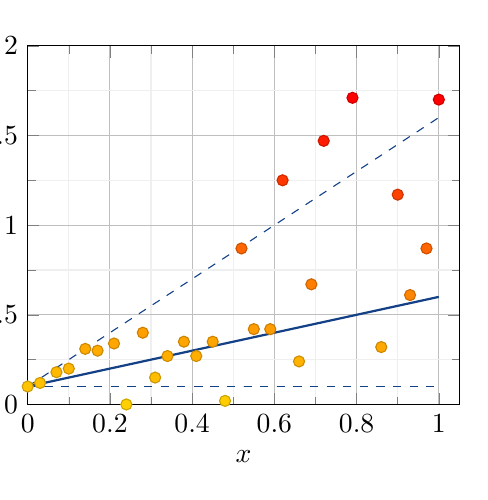
\begin{tikzpicture}[baseline,trim axis left]
    \begin{axis}[
       scale=0.8,
        xmin=0, xmax=1.05,
        ymin=0, ymax=2.0,
        xlabel={$x$},
        ylabel={$y$},
        grid=both,
        minor tick num=1,
        major grid style={lightgray},
        minor grid style={lightgray!25},
    ]
        \addplot+ [
            scatter, only marks
        ] coordinates {
    (0.0, 0.1) (0.03, 0.12) (0.07, 0.18) (0.1, 0.2) (0.14, 0.31) (0.17, 0.3) (0.21, 0.34) (0.24, -0.0) (0.28, 0.4) (0.31, 0.15) (0.34, 0.27) (0.38, 0.35) (0.41, 0.27) (0.45, 0.35) (0.48, 0.02) (0.52, 0.87) (0.55, 0.42) (0.59, 0.42) (0.62, 1.25) (0.66, 0.24) (0.69, 0.67) (0.72, 1.47) (0.76, -1.03) (0.79, 1.71) (0.83, -1.44) (0.86, 0.32) (0.9, 1.17) (0.93, 0.61) (0.97, 0.87) (1.0, 1.7)
        };
        \addplot [thick,
            mitblue,
            domain=0:1,
            samples=60,
        ]
            {0.5*x+0.1};
        \addplot [dashed,
            mitblue,
            domain=0:1,
            samples=60,
        ]
            {0.5*x+0.1+x};
            
              \addplot [dashed,
            mitblue,
            domain=0:1,
            samples=60,
        ]
            {0.5*x+0.1-0.5*x};  
    \end{axis}
    \end{tikzpicture}
    \end{column}
		\begin{column}{.5\textwidth}
     \begin{tikzpicture}[baseline,scale=1.5]
			% Input Layer
			%\foreach \i in {1,...,2}
			\node[input] (I-1) at (0,-1-0.5) {$x$};
			\node[input] (I-2) at (0,-2-0.5) {$1$};
			%\node[below of=I-3, node distance=0.8cm] {Entradas};
			%\node (label1) at (0,-3.5) {Entradas};
			
			% Output Layer
			%\foreach \i in {1,...,2}
			%\node[output] (O-\i) at (1,-\i-0.5) {$y_{\i}$};
			\node[output] (O-1) at (1,-1-0.5) {$\mu$};
			\node[output] (O-2) at (1,-2-0.5) {$\sigma^2$};
			%\node[below of=O-2, node distance=0.8cm] {Salidas};
			%\node (label2) at (1,-3.5) {Salidas};
			\node at (6,-1.7) {...}; % Elipsis
			\node at (6,-4.5) {}; % Spacing hack
			\node at (0.5,0.0)  {$y \sim \mathcal N(\mu,\sigma^2)$};
			
			% Connections
			\foreach \i in {1,...,2}
			\foreach \j in {1,...,2}
			\draw[line] (I-\i) -- (O-\j);
		\end{tikzpicture}
	\end{column}
	\end{columns}


\end{frame}

\begin{frame}
	\frametitle{Máxima Verosimilitud}
	%\framesubtitle{De la Predicción Puntual a la Distribución de Probabilidad}
	\begin{columns}[T]
		\begin{column}{.5\textwidth}
	\begin{tikzpicture}
	\begin{axis}[
		scale=0.5,
		no markers, domain=0:10, samples=100,
		axis lines*=left, xlabel=$x$, ylabel=$y$,
		every axis y label/.style={at=(current axis.above origin),anchor=south},
		every axis x label/.style={at=(current axis.right of origin),anchor=west},
		height=5cm, width=12cm,
		xtick=\empty, ytick=\empty,
		enlargelimits=false, clip=false, axis on top,
		grid = major
		]
		\addplot [very thick,cyan!50!black] {gauss(4,1)};
		\addplot [very thick,cyan!50!black] {gauss(6.5,2)};
		\draw [yshift=3cm](axis cs:4,0)  node [font=\small] {$\omega_1*\mathcal N(\mu_1,\sigma_1)+\omega_2*\mathcal N(\mu_2,\sigma_2)$} (axis cs:5.96,0);
		%\draw [yshift=3cm](axis cs:6.5,0)  node [font=\tiny] {$\mathcal N(\mu_2,\sigma_2)$} (axis cs:5.96,0);
	\end{axis}
	
\end{tikzpicture}
		\end{column}
		\begin{column}{.5\textwidth}
		 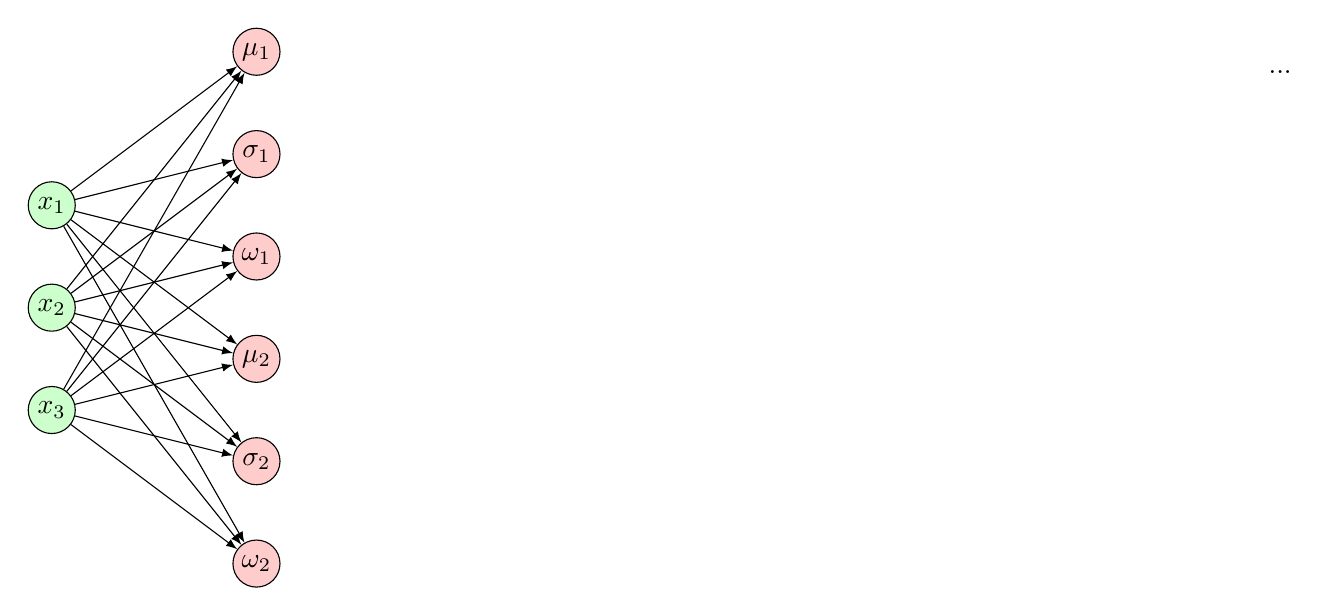
\begin{tikzpicture}[x=2.cm, y=1.0cm, >=stealth,scale=1.3]
		 	% Input Layer
		 	\foreach \i in {1,...,3}
		 	\node[input] (I-\i) at (0,-\i-2.0) {$x_{\i}$};
		 	%\node[below of=I-3, node distance=0.8cm] {Entradas};
		 	%\node (label1) at (0,-5.5) {Entradas};
		 	
		 	% Output Layer
		 	\node[output] (O-1) at (1,-1-0.5) {$\mu_1$};
		 	\node[output] (O-2) at (1,-2-0.5) {$\sigma_1$};
		 	\node[output] (O-3) at (1,-3-0.5) {$\omega_1$};
		 	\node[output] (O-4) at (1,-4-0.5) {$\mu_2$};
		 	\node[output] (O-5) at (1,-5-0.5) {$\sigma_2$};
		 	\node[output] (O-6) at (1,-6-0.5) {$\omega_2$};
		 	%\node[below of=O-2, node distance=0.8cm] {Salidas};
		 	%\node (label2) at (1,-5.5) {Salidas};
		 	\node at (6,-1.7) {...}; % Elipsis
		 	\node at (6,-4.5) {}; % Spacing hack
		 	
		 	
		 	% Connections
		 	\foreach \i in {1,...,3}
		 	\foreach \j in {1,...,6}
		 	\draw[line] (I-\i) -- (O-\j);
		 \end{tikzpicture}
			
		\end{column}
	\end{columns}

\end{frame}

% --- Diapositiva 3: Criterio de Máxima Verosimilitud (MLE) ---
\begin{frame}[shrink]
	\frametitle{El Principio de Máxima Verosimilitud}
	\framesubtitle{Formulación del Criterio (MLE)}
	\begin{itemize}
		\item Para cada ejemplo de entrenamiento \(x_i\), el modelo computa los parámetros de la distribución \(\theta_i = f[x_i, \phi]\).
		\item Idealmente, cada salida observada $y_i$ debería tener una \textbf{alta probabilidad} bajo la distribución \(Pr(y_i|\theta_i)\) que corresponde a \(x_i\).
		\item El objetivo es elegir los parámetros \(\phi\) que \textbf{maximizan la probabilidad conjunta} de todas las observaciones de entrenamiento:
		\begin{equation*}
			\hat{\phi} = \underset{\phi}{\operatorname{argmax}} \prod_{i=1}^{I} Pr(y_i|f[x_i, \phi]) \tag{5.1}
		\end{equation*}
		\item Esta expresión se conoce como el \textbf{criterio de máxima verosimilitud (MLE)}.
	\end{itemize}
\end{frame}

% --- Diapositiva 4: Supuestos y Log-Verosimilitud ---
\begin{frame}[shrink]
	\frametitle{El Principio de Máxima Verosimilitud}
	\framesubtitle{Supuestos Clave y la Log-Verosimilitud}
	\begin{itemize}
		\item \textbf{Supuestos Implícitos del MLE:}
		\begin{enumerate}
			\item Los datos son \textbf{independientes e idénticamente distribuidos (i.i.d.)}: Esto significa que la forma de la distribución \(Pr(y_i|x_i)\) es la misma para cada punto de datos, y las observaciones son independientes entre sí.
			\begin{equation*}
				Pr(y_1, \dots, y_I|x_1, \dots, x_I) = \prod_{i=1}^{I} Pr(y_i|x_i) \tag{5.2}
			\end{equation*}
		\end{enumerate}
		\item \textbf{Problema Práctico con el Producto:} El producto de muchas probabilidades pequeñas (cada \(Pr(y_i|x_i)\) es \(\le 1\)) puede resultar en un número extremadamente diminuto, lo que causa problemas de \textbf{precisión numérica}.
		\item \textbf{Solución: Maximizar la Log-Verosimilitud:}
		\begin{itemize}
			\item El logaritmo es una función \textbf{monotónicamente creciente}.
			\item Esto implica que maximizar una función \(g[z]\) es equivalente a maximizar \(\log(g[z])\). El máximo ocurre en la misma posición.
			\item \textit{Visualización (se podría usar TikZ):} Muestre una función \(g(z)\) y su \(\log(g(z))\), resaltando que los picos coinciden (similar a la Figura 5.2 del material).
			\item Por lo tanto, podemos maximizar la \textbf{log-verosimilitud}:
			\begin{equation*}
				\hat{\phi} = \underset{\phi}{\operatorname{argmax}} \sum_{i=1}^{I} \log [Pr(y_i|f[x_i, \phi])] \tag{5.3}
			\end{equation*}
			\item La ventaja clave es que convertimos un \textbf{producto en una suma}, lo que es numéricamente mucho más estable.
		\end{itemize}
	\end{itemize}
\end{frame}

% --- Diapositiva 5: Negativo de la Log-Verosimilitud (NLL) ---
\begin{frame}
	\frametitle{La Función de Pérdida Final: NLL}
	\framesubtitle{Minimizando el Negativo de la Log-Verosimilitud}
	\begin{itemize}
		\item Por convención en el aprendizaje automático, los problemas se formulan como \textbf{minimización de una función de costo}.
		\item Para transformar el criterio de máxima log-verosimilitud en un problema de minimización, simplemente lo \textbf{multiplicamos por menos uno}:
		\begin{equation*}
			\hat{\phi} = \underset{\phi}{\operatorname{argmin}} \left[ -\sum_{i=1}^{I} \log Pr(y_i|f[x_i, \phi]) \right] \tag{5.4}
		\end{equation*}
		\item Esta expresión define nuestra \textbf{función de pérdida final} $L[\theta]$.
	\end{itemize}
\end{frame}

% --- Diapositiva 6: Inferencia ---
\begin{frame}
	\frametitle{Inferencia: Obteniendo una Predicción}
	\begin{itemize}
		\item Una vez que el modelo ha sido entrenado y los parámetros \(\phi\) están optimizados, ¿cómo obtenemos una predicción para una nueva entrada $x$?
		\item El modelo no produce un valor $y$ directamente, sino una distribución de probabilidad \(Pr(y|f[x, \phi])\).
		\item A menudo, necesitamos una \textbf{estimación puntual} \(\hat{y}\) en lugar de una distribución completa. Esto se logra encontrando el valor de $y$ que \textbf{maximiza la probabilidad} de la distribución:
		\begin{equation*}
			\hat{y} = \underset{y}{\operatorname{argmax}} [Pr(y|f[x, \phi])] \tag{5.5}
		\end{equation*}
		\item Para la distribución normal univariada, el máximo de la distribución se encuentra en su \textbf{media} \(\mu\). Por lo tanto, para un modelo que predice la media, \(\hat{y} = f[x, \phi]\).
	\end{itemize}
\end{frame}

% --- Diapositiva 7: Receta para Construir Funciones de Pérdida ---
\begin{frame}
	\frametitle{Receta para Construir Funciones de Pérdida}
	\begin{block}{Pasos Clave basados en Máxima Verosimilitud (Sección 5.2)}
		Para un conjunto de datos de entrenamiento \(\{x_i, y_i\}\):
		\begin{enumerate}
			\item \textbf{Elegir una distribución de probabilidad} \(Pr(y|\theta)\) adecuada para el dominio de las predicciones $y$, con sus parámetros \(\theta\).
			\item \textbf{Configurar el modelo de aprendizaje automático} $f(x)$para que prediga uno o más de estos parámetros. Es decir, \(\theta = f[x, \phi]\) y por lo tanto \(Pr(y|\theta) = Pr(y|f[x, \phi])\).
			\item \textbf{Entrenar el modelo} encontrando los parámetros \(\phi\) que minimizan la función de pérdida del negativo de la log-verosimilitud sobre los pares de datos de entrenamiento \(\{x_i, y_i\}\):
			\begin{equation*}
				\hat{\phi} = \underset{\phi}{\operatorname{argmin}} \left[ L[\phi] \right] = \underset{\phi}{\operatorname{argmin}} \left[ -\sum_{i=1}^{I} \log [Pr(y_i|f[x_i, \phi])] \right] \tag{5.6}
			\end{equation*}
			\item \textbf{Realizar inferencia} para un nuevo ejemplo de prueba $x$. Esto puede ser devolviendo la distribución completa \(Pr(y|f[x, \phi])\) o el valor de $y$ donde esta distribución se maximiza (\(\hat{y}\)).
		\end{enumerate}
	\end{block}
\end{frame}

% --- Diapositiva 8: Ejemplo - Regresión Univariada (Pérdida de Mínimos Cuadrados) ---
\begin{frame}[shrink]
	\frametitle{Ejemplo: Regresión Univariada}
	\framesubtitle{Derivación de la Pérdida de Mínimos Cuadrados}
	\begin{itemize}
		\item \textbf{Objetivo:} Predecir una salida escalar \(y \in \mathbb{R}\) a partir de una entrada escalar $x$.
		\item \textbf{Distribución elegida:} La distribución normal univariada.
		\item \textbf{Función de Densidad de Probabilidad (PDF):}
		\begin{equation*}
			Pr(y|\mu, \sigma^2) = \frac{1}{\sqrt{2\pi\sigma^2}} \exp\left[-\frac{(y - \mu)^2}{2\sigma^2}\right] \tag{5.7}
		\end{equation*}
		\item \textbf{El modelo predice la media:} Sea \(\mu = f[x, \phi]\). Entonces, la probabilidad condicional es:
		\begin{equation*}
			Pr(y|f[x, \phi], \sigma^2) = \frac{1}{\sqrt{2\pi\sigma^2}} \exp\left[-\frac{(y - f[x, \phi])^2}{2\sigma^2}\right] \tag{5.8}
		\end{equation*}
	\end{itemize}
	\end{frame}
		
		% --- Diapositiva 9: Derivación de Mínimos Cuadrados (Continuación) ---
		\begin{frame}[shrink]
			\frametitle{Ejemplo: Regresión Univariada}
			\framesubtitle{Derivación de la Pérdida de Mínimos Cuadrados (Continuación)}
			\begin{itemize}
				\item Aplicando el negativo de la log-verosimilitud (Ecuación 5.4):
				\begin{align*}
					L[\phi] &= -\sum_{i=1}^{I} \log \left[Pr(y_i|f[x_i, \phi], \sigma^2)\right] \tag{5.9} \\
					&= -\sum_{i=1}^{I} \log \left[ \frac{1}{\sqrt{2\pi\sigma^2}} \exp\left(-\frac{(y_i - f[x_i, \phi])^2}{2\sigma^2}\right) \right] \\
					&= -\sum_{i=1}^{I} \left[ \log \left(\frac{1}{\sqrt{2\pi\sigma^2}}\right) - \frac{(y_i - f[x_i, \phi])^2}{2\sigma^2} \right] \\
					&= \sum_{i=1}^{I} \left[ \frac{(y_i - f[x_i, \phi])^2}{2\sigma^2} - \log \left(\frac{1}{\sqrt{2\pi\sigma^2}}\right) \right]
				\end{align*}
				\item Al minimizar $L[\theta]$, podemos ignorar los términos que no dependen de \(\phi\) (como \(\sigma^2\), si se asume constante) y el factor constante \(1/(2\sigma^2)\):
				\begin{equation*}
					\underset{\phi}{\operatorname{argmin}} L[\phi] \propto \underset{\phi}{\operatorname{argmin}} \sum_{i=1}^{I} (y_i - f[x_i, \phi])^2 \tag{5.10}
				\end{equation*}
				\item El resultado es la conocida \textbf{función de pérdida de Mínimos Cuadrados}:
				\begin{equation*}
					L[\phi] = \sum_{i=1}^{I} (y_i - f[x_i, \phi])^2 \tag{5.11}
				\end{equation*}
				\item Esto demuestra cómo la pérdida de mínimos cuadrados surge naturalmente de asumir que los errores son independientes y están distribuidos normalmente alrededor de la predicción del modelo.
			\end{itemize}
			\end{frame}
				
				% --- Diapositiva 10: Conclusión ---
				\begin{frame}
					\frametitle{Conclusión}
					\begin{itemize}
						\item Las \textbf{funciones de pérdida} son el motor del entrenamiento en el aprendizaje supervisado, transformando la "bondad" de un modelo en una cantidad optimizable.
						\item El \textbf{Principio de Máxima Verosimilitud} provee un marco teórico robusto para la construcción de estas funciones, al ver el modelo como un predictor de distribuciones de probabilidad.
						\item La utilización de la \textbf{log-verosimilitud negativa} resuelve problemas de estabilidad numérica y convierte la maximización en una minimización.
						\item La \textbf{pérdida de mínimos cuadrados} es un ejemplo clásico que surge directamente de asumir una distribución normal para los errores.
						\item La elección de la función de pérdida correcta es crucial y depende del tipo de problema (regresión, clasificación, etc.) y de las suposiciones sobre los datos.
					\end{itemize}
				\end{frame}
				
				% --- Diapositiva Final: Preguntas ---
	
\end{document}